\documentclass[10pt,mathserif]{beamer}
\setbeamertemplate{navigation symbols}{}
%\documentclass[handout]{beamer} % use this instead for handouts
\pdfoutput=1
%% Non beamer specific
\usepackage{amssymb}
\usepackage{wasysym}
\usepackage{epsfig,psfrag}
\usepackage{mathrsfs}
\usepackage{hyperref}
\usepackage{bm,amsmath}%  allow additional maths symbols
\usepackage{hyperref,url}     % for hyperreferences
\usepackage{graphicx}
\usepackage{subfigure}
\usepackage{framed}
\def\emptyline{\vspace{12pt}}
%% Beamer specifics

\graphicspath{{figs_pdf/}}

\usepackage{beamerthemeBoadilla}

\beamertemplateshadingbackground{white}{white}  % the 2 background colours
%\beamertemplatetransparentcovereddynamic  % covered items only grayed out

%\setbeamertemplate{headline}    % switch OFF headline 
%\setbeamertemplate{footline}    % switch OFF footline 
% RRK %%%%%%%%%%%%%%%%%%%%%%%%%%%%%%%%%%%%%%%%%%%%%%%%%%


\newcommand{\mathd}{\mathrm{d}}
\newcommand{\mathe}{\mathrm{e}}


\newcommand{\imag}{\mathrm{i}}

\newcommand{\vecuhat}{\widehat{\bm{u}}}
\newcommand{\vecnhat}{\widehat{\bm{n}}}
\newcommand{\hatu}{\widehat{u}}
\newcommand{\hatn}{\widehat{n}}
\newcommand{\vecx}{\bm{x}}

\newcommand{\vecv}{\bm{\mathrm{v}}}
\newcommand{\vecu}{\bm{\mathrm{u}}}

\newcommand{\myra}{\mathrm{Ra}}
\newcommand{\mypr}{\mathrm{Pr}}
\newcommand{\mynu}{\mathrm{Nu}}
\newcommand{\Tamb}{T_{\mathrm{amb}}}
\newcommand{\Thot}{T_{\mathrm{hot}}}
\newcommand{\Tcold}{T_{\mathrm{cold}}}


%\newcommand{\kappaf}{\kappa_{\mathrm{f}}}
%\newcommand{\nuf}{\nu_{\mathrm{f}}}

\newcommand{\kappaf}{\kappa_2}
\newcommand{\nuf}{\nu_2}
\newcommand{\kf}{k_2}
\newcommand{\alphaf}{\alpha_2}
\newcommand{\mypraf}{\mathrm{Pr}_2}

%\newcommand{\kappaa}{\kappa_{\mathrm{a}}}
%\newcommand{\nua}{\nu_{\mathrm{a}}}

\newcommand{\kappaa}{\kappa_3}
\newcommand{\nua}{\nu_3}
\newcommand{\ka}{k_3}
\newcommand{\alphaa}{\alpha_3}
\newcommand{\mypra}{\mathrm{Pr}_3}

\newcommand{\Je}{J_E}

\newcommand{\emphlon}[1]{\textcolor{blue}{\textbf{#1}}}

\definecolor{mygray}{HTML}{F8F8F9}


\begin{document}

%\input ../macros.tex

%%%%%%%%%%%%%%%%%%%%%%%%%%%%%%%%%%%%%%%%%%%%%%%%%%%%%%%%%%%%%%%%%%%%%%%%%%%

%%%% Setup Title Page %%%%%%%%%%%%%%%%%%%%%%%%%%%%%%%%%%%%%%%%%%%%%%%%%%%%%
\title[Modelling the fluid orientation dynamics using SDE]{Modelling the Lyapunov exponent of a tracer gradient using a stochastic differential equation.}
\author[]{
Ian Towey
}
\date{\today}

\institute[]{
Msc Data and Computational Science\\
School of Mathematics and Statistics, University College Dublin
}
%%%%%%%%%%%%%%%%%%%%%%%%%%%%%%%%%%%%%%%%%%%%%%%%%%%%%%%%%%%%%%%%%%%%%%%%%%%

\begin{frame}
    \titlepage
\end{frame}

\section{Context}

\begin{frame}{Context of work}

\begin{columns}[t]						% the [t] option aligns the column's content at the top
\begin{column}{0.64\linewidth}
\visible<1->{Modeling chaotic mixing of tracer:
%
%
\begin{itemize}
\item Numerical Simulation of two-dimensional turbulence.
%
%
\item Model 2D vorticity using a system of stochastic differential equations.
\item Use the equilibrium solution of the SDEs corresponding Fokker-Planck PDE to find the PDF of the orientation angles and growth rate (Lyapunov exponent).
\item Compare the PDF of the orientation angles from the vorticity simulation and the SDE model
\end{itemize}
}
%
%
\visible<2->{
\begin{framed}
\[
\frac{\partial \omega}{\partial t} + \mathbf{u} \cdot \nabla \omega = 0 + (-1)^p \nu_p \nabla^{2p} \omega + \nabla \times \mathbf{F} - \nabla \times \mathbf{D} 
\] 
\end{framed}
}
\end{column}
%
%
%
%
\end{columns}
%
%
%
%
%
\end{frame}

\section{Mathematical modelling}


\begin{frame}{Numerical simulation of 2D Vorticity/advection-diffusion}
\begin{itemize}
\item \visible<1->
{Using pseudospectral methods to numerically solve Vorticity and advection-diffusion equations.}

\item \visible<2->
{Extract emperical PDF of orientation angles and growth rates by averaging over histograms}
\end{itemize}
\vskip 0.1in
\visible<3->{
Two proposed solutions, both involving passive cooling methods:
%
\begin{itemize}
\item \emphlon{Convective cooling}, which exploits the adverse temperature gradient created by the pipe and its surroundings, in the presence of gravity, further enhanced by suspending \emphlon{phase-changing bubbles} in the working fluid.
}
%
\visible<4->{
\item \emphlon{A sieve cooler}
\end{itemize}
Both approaches can be placed in the same generic mathematical framework.
}
\end{frame}


\begin{frame}{Modelling Approach}

\visible<1->{
\begin{columns}[t]						% the [t] option aligns the column's content at the top
\begin{column}{0.45\linewidth}
\begin{itemize}
\item Region 1 -- closed to the pipe surface.  Contains the TEG.
\item Region 2 -- contains the cooling device.
\item Region 3 -- zone where cooler interacts with ambient air.
\end{itemize}
%
\end{column}
%
%
%
%
\begin{column}{0.65\linewidth}
\begin{figure}
\hspace{-0.5in}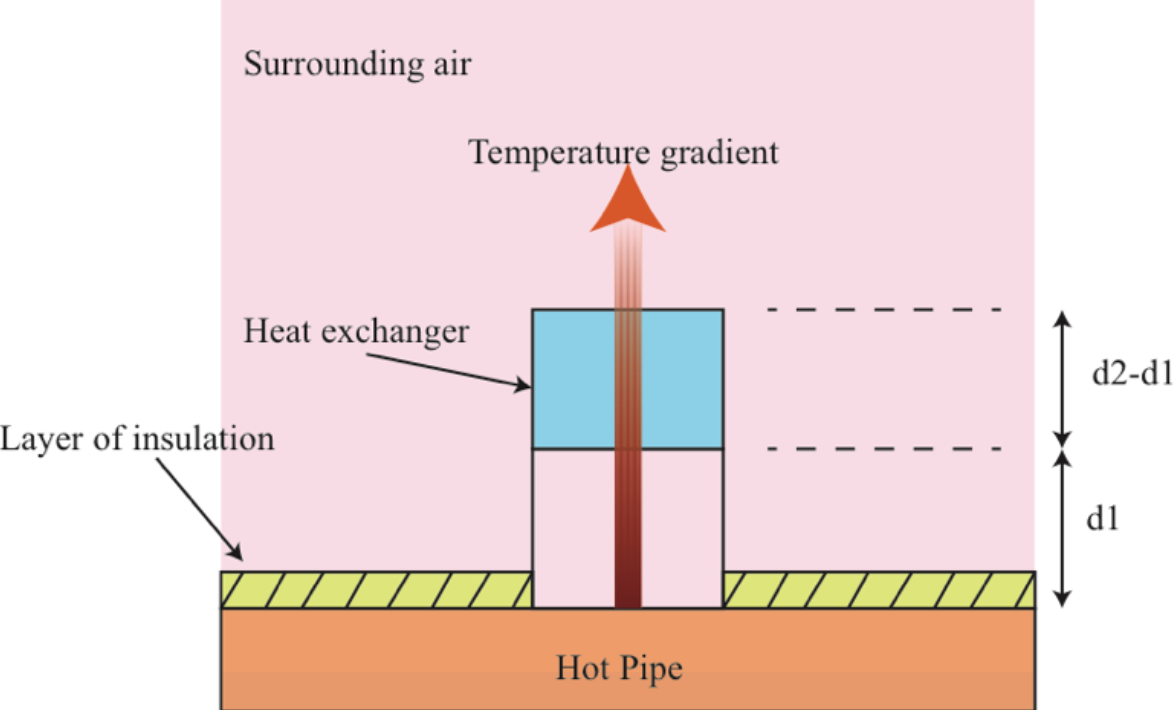
\includegraphics[width=0.9\linewidth]{figs_pdf/schematic1}
%\caption{}
\end{figure}
\end{column}
\end{columns}
}
%
%
\vspace{0.3in}
\visible<2->{
For convective cooling, the adverse temperature gradient is maintained by gravity, meaing that the cooler is mounted on top of the pipe -- \emphlon{Rayleigh--B\'enard convection}
}
%
\end{frame}


\begin{frame}{Region 1}

\visible<1->{
\begin{itemize}
\item Region closed to pipe surface, in contact with pipe through patch of area $A$.
\item Pipe maintained at constant temperature $T_0=60^\circ\mathrm{C}$
\item Otherwise, pipe is assumed to be \emphlon{fully insulated}
\item TEG located in region 1
\end{itemize}
}
%
%
\visible<2->{
\begin{framed}
\emphlon{Region 1 is modelled as a thermally conducting region:}
%
\begin{itemize}
\item TEG can be assigned an `effective' thermal conductivity $k_1$ taking account of thermal conduction and heat generation/consumption due to thermoelectric effects, with $k_1\approx 1\,\mathrm{W/(m\,K)}$
\item Size of region is $d_1$, with $d_1\geq d_{TEG}$.  Values with $d_1>d_{TEG}$ could be achieved by embedding the TEG in a medium that is conductivity-matched to the TEG.
\end{itemize}
%
\end{framed}
}
%
%
%
\end{frame}


\begin{frame}{Region 2}

\visible<1->{
\begin{columns}[t]						% the [t] option aligns the column's content at the top
\begin{column}{0.45\linewidth}
\begin{itemize}
\item Region 2 contains the cooling device, either convective cooler or sieve cooler
\item Main focus -- \emphlon{convective cooling}
\end{itemize}
%
\end{column}
%
%
%
%
\begin{column}{0.65\linewidth}
\begin{figure}
\hspace{-0.4in}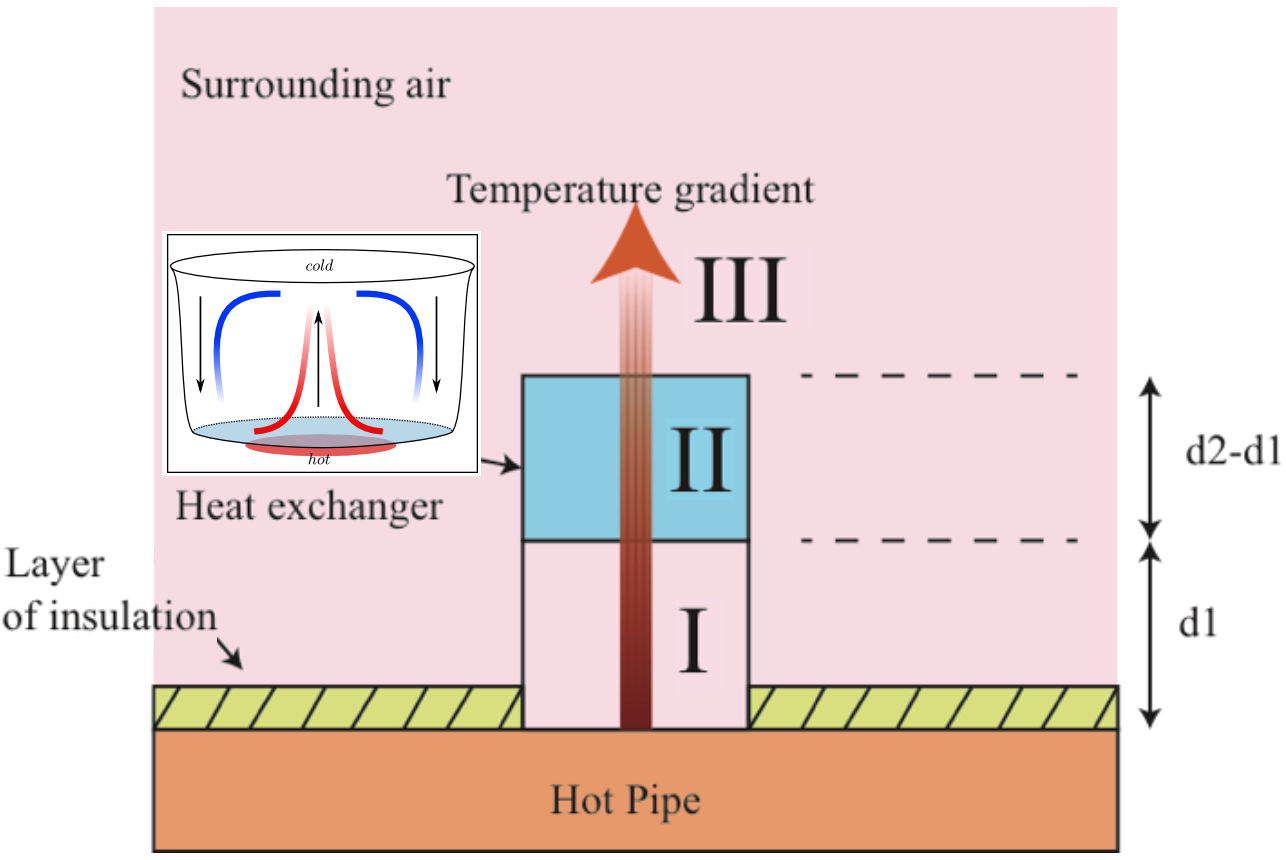
\includegraphics[width=0.9\linewidth]{figs_pdf/schematic1_rb}
%\caption{}
\end{figure}
\end{column}
\end{columns}
}
%
%
\vspace{0.1in}
%
%
%
\visible<2->{
\vspace{-0.2in}
\begin{framed}
Using the theory of Rayleigh--B\'enard convection, we shall compute an effective conductivity for region 2, $k_{2,\mathrm{eff}}=k_2\,\mynu$, where
%
\begin{itemize}
\item $k_2$ is the ordinary thermal conductivity,
\item $\mynu$ is the \emphlon{Nusselt number}, defined in what follows.
\end{itemize}
%
\end{framed}
}
%
%
%
\end{frame}

\begin{frame}{Region 3 and matching}

\visible<1->{
\begin{itemize}
\item Region 3 is just the surrounding air with thermal conductivity $k_3$.
\item In each region, the heat equation
%
%
\[
k_{i\,\mathrm{eff}}\left(\mathd T/\mathd x\right)=J
\] is solved for the temperature $T$ ($x=0$ is the pipe surface).    Here, $k_{i\,\mathrm{eff}}$ is the  thermal conductivity (effective or otherwise) appropriate for each layer and $J_E$ is the heat flux.
}
%
%
\visible<2->{
\item \emphlon{Matching conditions} at the region boundaries close the resulting system of equations.
\end{itemize}
%
%
\begin{figure}
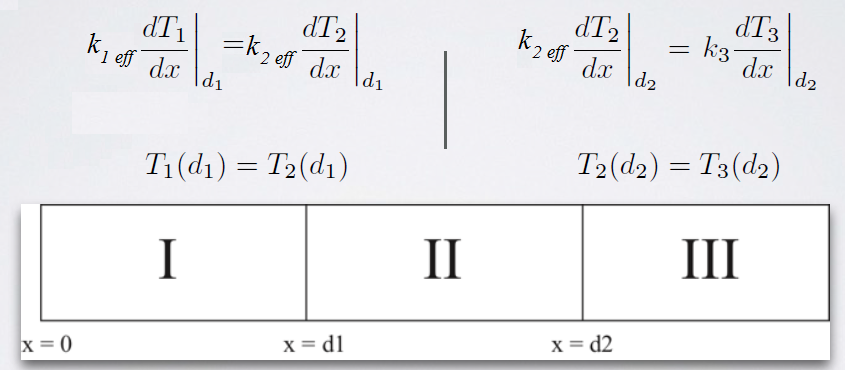
\includegraphics[width=0.7\linewidth]{figs_pdf/matching}
%\caption{}
\end{figure}
}
%
%
%
\end{frame}




\section{Convection}


\begin{frame}{Rayleigh--B\'enard convection}
\visible<1->{
\begin{itemize}
\item Refers to the problem of `a fluid heated from below'
\item Adverse temperature gradient formed due to gravity -- hot fluid ends up sitting on the bottom
\item Convection pattern sets in to redistribute the hot fluid
\item Leads to enhanced heat transfer
\end{itemize}
}

\visible<2->{
\begin{framed}
Convection sets in above a critical value of the \emphlon{Rayleigh number}
%
\[
\myra=\frac{g\alpha (\Thot-\Tcold)\ell^3}{\nu\kappa},
\]
%
\vspace{-0.2in}
\begin{small}
\begin{itemize}
\item $g$ is the acceleration due to gravity
\item $\alpha$ is the thermal expansion coefficient in $\mathrm{K}^{-1}$
\item $\Thot-\Tcold$ is the temperature difference across region 2
\item $\ell=d_2-d_1$ is the vertical extent of region 2
\item $\kappa$ is the thermal diffusivity in $\mathrm{m^2}/\mathrm{s}$
\end{itemize}
\end{small}
%
Typically, \emphlon{$\myra \apprge 10^3-10^4$} for the onset of convection.
\end{framed}
}
%
\end{frame}





\begin{frame}{Rayleigh--B\'enard convection -- enhanced heat transfer}

\visible<1->{
Fluid motion enhances heat transfer.  This is quantified by the \emphlon{Nusselt number}
%
\[
\mynu=\frac{\langle \int_0^1 \left(wT-\kappa_2\frac{\partial T}{\partial x}\right)\mathd x\rangle}{\kappa_2\left(\Thot-\Tcold\right)}.
\]
}
%
%
\visible<2->{
Not known \textit{a priori} but useful correlations exist from experiments / DNS:
%
\[
\mynu=\begin{cases} 0.54\,\myra^{1/4},& 10^3\leq \myra\leq 10^7,\qquad \mypr\geq 0.7,\\
                    0.15\,\myra^{1/3},& 10^7\leq \myra\leq 10^{11},\qquad \text{ all}\mypr,
										\end{cases}
\]
%
where $\mypr=\nu/\kappa$ is the \emphlon{Prandtl number}.
}

\end{frame}

\begin{frame}{Rayleigh--B\'enard convection -- added phase change}

\visible<1->{
To further enhance the heat transfer over and above what is achievable by ordinary RBC, it is proposed to use a working fluid such that
%
\begin{itemize}
\item The fluid is a liquid-phase suspension mixed in with gas-phase boiling bubbles of the same substance.
\item The fluid is maintained close to the boiling temperature.
\item The bubbles condense on the cold plate, are transported to the hot plate, where they (partially) evaporate, releasing latent heat.
\item This further enhances the heat transfer.
\end{itemize}
%
}
%
%
\visible<2->{
\begin{framed}
Enhanced heat transfer is quantified by a modified Nusselt-number correlation obtainable from DNS studies in the literature:
%
\[
\mynu=A(\xi)\myra^{\gamma(\xi)},\qquad \xi=\frac{\Thot-T_{\mathrm{sat}}}{\Thot-\Tcold}
\]
%
where $A(\xi)\approx 1+66.31\xi$ and $\gamma(\xi)=(1/3)-0.26\xi$, and $0\leq \xi\leq 0.5$.
\end{framed}
}

\end{frame}


\begin{frame}{Convection in the plume}



\visible<1->{
\begin{columns}[t]						% the [t] option aligns the column's content at the top
\begin{column}{0.55\linewidth}
Recall, region 3 consists of the ambient air in contact with the surface of the convective cooler.  This region can therefore be modelled as a \emphlon{convective plume}.
%
%
\end{column}
%
%
%
%
\begin{column}{0.45\linewidth}
\begin{figure}
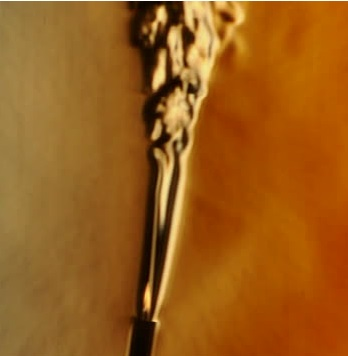
\includegraphics[width=0.9\linewidth]{figs_pdf/plume}
%\caption{}
\end{figure}
\end{column}
\end{columns}
}
%
%
\end{frame}

\begin{frame}{Convection in the plume -- model}

\visible<1->{
We have taken the plume model of Morton, Taylor, and Turner and added a thermal boundary layer (to allow for a non-pointlike heat source).  Result is an expression for the heat flux into region 3:
%
\[
J_E=\mu_0\frac{\theta_0 k_3}{R_0}\left(\myra_3\mypr_3\right)^{1/7},\qquad \myra_3=\frac{g\alpha\theta_0 R_0^3}{\kappa_3\nu_3},\qquad \mypr_3=\frac{\nu_3}{\kappa_3}
\]
%
}
%
%
where $\theta_0=\Tcold-\Tamb$, \visible<2->{and
%
\begin{itemize}
\item $\nua=1.568\times 10^{-5}\,\mathrm{m^2/s}$
\item $\kappaa=1.9\times 10^{-5}\,\mathrm{m^2/s}$, hence $\mypr=0.8253$
\item $\alphaa=3.43\times 10^{-3}\,\mathrm{K^{-1}}$,
\item $R_0=10^{-2}\,\mathrm{m}=1\,\mathrm{cm}$ -- patch radius
\item $\Tamb=20^\circ\,\mathrm{C}$, $\Thot=60^\circ\,\mathrm{C}$  %hence $\theta_0=40^\circ\,\mathrm{C}$
\item $\mu=0.14$
\end{itemize}
}
%
%
\end{frame}


\begin{frame}{Upper bound}
\visible<1->{
In practice, $\theta_0$ has to be found by matching across the regions.  But this is not necessary if we want to find an \emphlon{upper bound} on the temperature drop achievable across region 1, since $\theta_0\leq \Tamb-T_0$, hence
%
\[
\frac{\left(\Delta T\right)_{\text{Reg\,1}}}{d_1}\leq
\mathrm{max}\left[\frac{\left(\Delta T\right)_{\text{Reg\,1}}}{d_1}\right]:=
\mu_0\frac{k_3}{k_1}\frac{(T_0-\Tamb)}{R_0}\left(\myra_{T,3}\,\mypr_3\right)^{1/7}.
\]
%
}
%
\visible<2->{
Hence,
%
\[
\frac{\left(\Delta T\right)_{\text{Reg\,1}}}{d_1}\leq  \frac{k_3}{k_1}\times 1.5101\times 10^3\,\mathrm{K/m}.
\]
}
\visible<3->{
But $k_3/k_1=k_{\mathrm{air}}/k_{TEG,\mathrm{eff}}=O(10^{-2})$, meaning that
%
\[
\frac{\left(\Delta T\right)_{\text{Reg\,1}}}{d_1}\apprle 10\,\mathrm{K/m}.
\]
This is off target -- heat transfer into the plume gives a very low \emphlon{limiting value} on the region-1 temperature gradient achievable.
}
\end{frame}


\section{Two-layer model}


\begin{frame}{Reduction to two-layer model}

\begin{itemize}
\item We can sidestep the limiting value by imposing that the cold plate be temperature-matched to the ambient environment -- \emphlon{two-layer model}.
\item Solution temperature profiles read
%
\begin{align*}
T_1&=T_0-\frac{\Je x}{k_1},\\
T_2&=T_0-\frac{\Je d_1}{k_1}-\frac{\Je}{k_2\mynu}(x-d_1).
\end{align*}
%
and we require $T_2(d_2)=\Tamb$.
%
\item The matching procedure is \emphlon{nonlinear}, as $\mynu$ depends on $T_2(d_2)-T_2(d_1)$.
\end{itemize}
\end{frame}

\begin{frame}{Parameter study -- question to be asked}

\begin{itemize}
\item  We fix
%
\[
\left(\Delta T\right)_{\text{Reg 1}}=d_1\left(\mathd T/\mathd x\right)_*
\]
%
and ask the question, for what values of $\ell$ can $T_2(d_2)=\Tamb$ be achieved?  
\item In practice, we want to know the value of $(\Delta T)_{\mathrm{tot}}=\Tamb-T_0$ for a given value of $\ell$ -- \emphlon{can  $(\Delta T)_{\mathrm{tot}}=40\,\mathrm{K}$ be achieved for a sensible value of $\ell$?}
\item We have other constraints on region 1 -- temperature drop in region 1 can be at most the total temperature drop:
%
\[
d_1\leq \frac{\left(\Delta T\right)_{\mathrm{tot}}}{\left(\mathd T/\mathd x\right)_*},
\]
hence
%
\[
d_{TEG}\leq d_1\leq \frac{\left(\Delta T\right)_{\mathrm{tot}}}{\left(\mathd T/\mathd x\right)_*},
\]
\end{itemize}
%
\end{frame}

\begin{frame}{Parameter study -- no phase change}
%
We fix
\begin{itemize}
\item $d_1=2\times 10^{-5}\,\mathrm{m}$--$\left[40\,\mathrm{K}/(2.5\times 10^5\,\mathrm{K/m})\right]=1.6\times 10^{-4}\,\mathrm{m}$
\item $k_1=1\,\mathrm{W/(m\,K)}$ -- an estimated `effective' value for the TEG.
\item $k_2=0.6\,\mathrm{W/(m\,K)}$ -- this is the value for water but should be broadly similar for many working fluids.
\end{itemize}
%
\vspace{-0.08in}
\begin{figure}
	\centering
		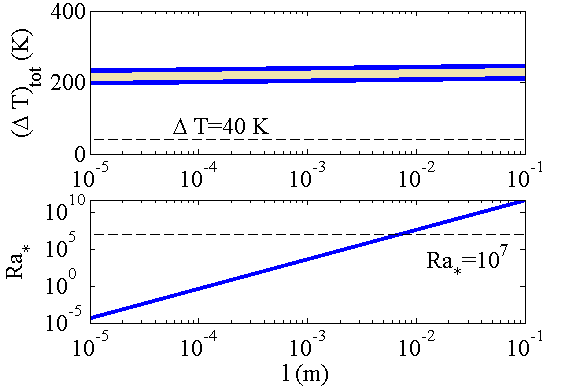
\includegraphics[width=0.7\textwidth]{size_L_singlephase}
	\label{fig:size_L_singlephase}
\end{figure}
\end{frame}


\begin{frame}{Parameter study -- with phase change}
\begin{figure}
	\centering
		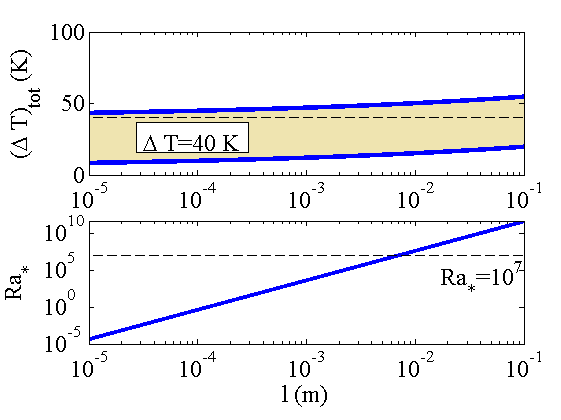
\includegraphics[width=0.9\textwidth]{size_L_twophase}
	\label{fig:size_L_singlephase}
\end{figure}
\end{frame}


\begin{frame}{Electrical circuit analogy}
\visible<1->{
Re-write $J_E\equiv I$, $R_1=d_1/k_1$, and the region-1 temperature drop as $\Delta V_1$.  Then,
%
\[
\Delta V_1=I R_1\qquad\text{(Ohm's Law)}.
\]
%
}
%
%
\visible<2->{
Region 2 is a nonlinear resistor, with
%
\[
\Delta V_2=I R_2,\qquad R_2=\frac{\ell}{k_2}\frac{1}{\mynu}.
\]
$\mynu$ (hence $R_2$) depends on $I$:
%
\[
R_2=R_{20}(I/I_0)^{-c_2/(1+c_2)},\qquad R_{20},\,I_0=\text{Constants}
\]
}
%
%
\visible<3->{
Total temperature drop is
%
\[
\Delta V=\Delta V_1+\Delta V+2=I\left[R_1+R_{20}\left(I_0/I\right)^{c_2/(1+c_2)}\right]
\]
%
%
And we want to know for a given $I$, \emphlon{what values of the resistances give us the required total temperature drop $\Delta V$?}
}
\end{frame}

\section{Sieve cooler}

\begin{frame}{The sieve cooler}
\begin{itemize}
\item A rectangular metal of similar cross
section as the TEG, but with thickness $d_2 = 1\,\mathrm{mm}$.
\item A large number of tiny holes are punctured in the cooler
converting it into a sieve. In a preferred embodiment the holes are
filled with a material of extremely high conductivity.
\item We have shown that such a composite can cool the TEG to the
desired temperature with reasonable physical parameters.
\end{itemize}
\end{frame}

\begin{frame}{The sieve cooler -- modelling I}

\begin{columns}[t]						% the [t] option aligns the column's content at the top
\begin{column}{0.65\linewidth}
%
%
\begin{itemize}
\item The number $N$ and radius $R$ of the holes are scaled according to
$N = |\log \epsilon|$,  $R = \alpha\epsilon$.

Here $\epsilon$ is a small parameter that the engineers will need to select.
\item Deep mathematical analysis (Kac, Ozawa, ...) of the small-$\epsilon$ limit
shows that in the presence of such hole distribution, the spectrum
of the Laplacian is shifted by $O(\alpha)$.
\item This is equivalent to $O(\alpha)$ heat removal. Notice that in this scaling,
although the heat removal is significant, the total volume of the
holes is very small.
\end{itemize}
%
\end{column}
%
%
%
%
\begin{column}{0.4\linewidth}
\begin{figure}\begin{center}
\hspace{-0.2in}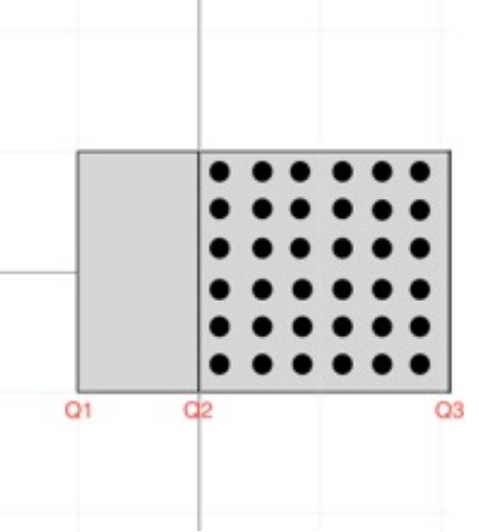
\includegraphics[width=0.9\linewidth]{figs_pdf/metal_plate}
%\caption{}
\end{center}
\end{figure}
\end{column}
\end{columns}
\end{frame}



\begin{frame}{The sieve cooler -- modelling II}

\begin{itemize}
\item The resulting model equations read
%The underlying equations are:
\begin{align*}
\frac{\mathd^2 T_1}{\mathd x^2}&=0,\qquad x\in (0,d_1), \\
\frac{\mathd^2T_2}{\mathd x^2} - \underbrace{\mu^2 T_2}_{\text{Sieve cooler}}&=0,\qquad x\in (d_1, d_2).
\end{align*}
%
\item The parameter $\mu^2$ measures the heat removal, and is determined  from the number and radius of the holes. It is the same as the spectrum shift of the Laplacian in this perforated domain:
\begin{equation*}
\mu^2:= 2 \pi \alpha/|\Omega|. 
\end{equation*}
%
\item 
Notice that the equations are an averaged (or homogenized) model for heat transfer in the cooler, that already takes into account the many tiny holes filled with highly conductive material.
\item This model can be embedded into our previous `matching' framework -- the results indicate that the desired temperature gradient can be achieved by the sieve cooler also.
\end{itemize}

\end{frame}

\section{Conclusions}

\begin{frame}
\frametitle{Summary / Conclusions I}
Using the theory of Rayleigh--B\'enard convection with phase change, we can give concrete answers to most of the questions posed at the start of the study group:
%
%\setbeamercolor{normal text}{fg=mygray,bg=}
%\setbeamercolor{alerted text}{fg=black,bg=}
%\usebeamercolor{normal text}
\setbeamercovered{transparent}
%
%\begin{itemize}
\begin{itemize}[<+>]
%\item \alert<+> 
\item {Is such a system [enhanced heat transfer with phase-changing convective cells] thermodynamically  feasible?

{\emph{Yes -- provided the cell is temperature-matched to the surroundings}}
}

%\item \alert<+> 
\item {What performance/size enhancements might be expected compared
to metallic cooling fins?

{\emph{We have not yet quantified performance enhancements but can say that the size of the cell can be made smaller than that for fins: $<1\,\mathrm{cm}$ compared to $4\,\mathrm{cm}$ for fins.}}
}

%\item \alert<+> 
\item{ What properties should the working fluid possess?

{\emph{The fluid should be a suspension of liquid phase surrounding phase-changing bubbles of the same substance.  The bubbles should be maintained near the boiling point.  The boiling point should therefore be between $\Tamb=20^\circ\mathrm{C}$ and $T_0=60^\circ\mathrm{C}$.  The Rayleigh number must be sufficiently large so as to ensure self-sustaining convection (ideally $\myra\geq O(10^4)$).}}
}



\end{itemize}
\end{frame}


\begin{frame}
\frametitle{Summary / Conclusions II}
%\setbeamercolor{normal text}{fg=mygray,bg=}
%\setbeamercolor{alerted text}{fg=black,bg=}
%\usebeamercolor{normal text}
\setbeamercovered{transparent}


%\begin{itemize}
\begin{itemize}[<+>]
%\item \alert<+> 
\item{What are the practical candidates for such a fluid?

{\emph{We don't know yet, but the search can be narrowed by looking at which fluids give the required phase-change, Nusselt number, and Rayleigh number characteristics.}}}

%\item \alert<+>
\item{What pressure should the closed system work at?

{\emph{This can be inferred from the phase diagram once the boiling temperature is specified; the latter must be between $\Tamb=20^\circ\mathrm{C}$ and $T_0=60^\circ\mathrm{C}$}}}

%\item \alert<+>
\item{What size and shape should the vessel be?

{\emph{The size and shape should be chosen so as to maximize the Nusselt number for a given Rayleigh number -- this can be explored further using the existing literature on convection.}}}

%\item \alert<+>
\item{Can the system self-start and under what conditions?

{\emph{Yes, convection self-starts once the critical Rayleigh number is attained.  However, it can take minutes for the convection to become fully developed.  This is an important consideration for using this kind of device.}}}

\end{itemize}
\end{frame}


\begin{frame}
\frametitle{Summary / Conclusions III}

%\setbeamercolor{normal text}{fg=mygray,bg=}
%\setbeamercolor{alerted text}{fg=black,bg=}
%\usebeamercolor{normal text}
\setbeamercovered{transparent}
%

%\begin{itemize}
\begin{itemize}[<+>]

%\item \alert<+>
\item{ Such a system will need to move the liquid phase back to the
evaporation site, how does the energy required to do this effect
the efficiency of the system? Will it impact scale?

{\emph{Because the device is entirely passive -- powered by the adverse temperature gradient -- no energy source is needed to move the liquid phase back to the evaporation site.  The boiling bubbles are carried around the cell by the convective velocity field.  There are also no impacts on the scale of the device.}}
}

%\item \alert<+>
\item{ Ideally, the hot-water pipe should be fully insulated with the
TEG/Cooler puncturing the insulation thereby providing a leakage path. What would be the impact of using
uninsulated pipes?

{\emph{Interaction with the environment (as in the three-region model) severely hampers the functionality of the cooling device.  Therefore, appropriate insulation (and in other parts of the device, temperature-matching) would appear to be essential.}}
}

%\item \alert<+>
\item{Is it more appropriate to re-design the TEG to match constraints
of a predefined heat-source (water-pipe)and working fluid?

{\emph{This would not seem to be necessary.  There is already some flexibility concerning the scale of region 1 -- this can be increased by embedding the TEG in a medium that is conductivity-matched to the TEG itself.}}
}
\end{itemize}
\end{frame}

\begin{frame}
\frametitle{Acknowledgements}
This work was carried out on foot of a project presented by Analog Devices at the 118th ESGI in July 2016.  Contributing participants at the study group were 
%
David Burton, 
Denis Flynn, 
James Gleeson, 
Andrew Gloster, 
Stephen O'Hara, 
Gary O'Keeffe, 
Lennon \'O N\'araigh, 
Jacob Rubenstein, and 
Shishir Suresh.
\end{frame}
\end{document}



\end{itemize}
\end{frame}

